%%%%%%%%%%%%%%%%%%%%%%%%%%%%%%%%%%%%%%%%%%%%%%%%%%%%%%%%%%%%%%%%%%%%%%%%%%%%%%%%
%%%%%%%%%%%%%%%%%%   Vorlage für eine Abschlussarbeit   %%%%%%%%%%%%%%%%%%%%%%%%
%%%%%%%%%%%%%%%%%%%%%%%%%%%%%%%%%%%%%%%%%%%%%%%%%%%%%%%%%%%%%%%%%%%%%%%%%%%%%%%%

% Erstellt von Maximilian Nöthe, <maximilian.noethe@tu-dortmund.de>
% ausgelegt für lualatex und Biblatex mit biber

% Kompilieren mit 
% lualatex dateiname.tex
% biber dateiname.bcf
% lualatex dateiname.tex
% lualatex dateiname.tex
% oder einfach mit:
% make

\documentclass[
  tucolor,
  BCOR=12mm,     % 12mm binding corrections, adjust to fit your binding
  parskip=half,  % new paragraphs start with half line vertical space
  open=any,      % chapters start on both odd and even pages
  cleardoublepage=plain,  % no header/footer on blank pages
]{tudothesis}


% Warning, if another latex run is needed
\usepackage[aux]{rerunfilecheck}

% just list chapters and sections in the toc, not subsections or smaller
\setcounter{tocdepth}{1}

%------------------------------------------------------------------------------
%------------------------------ Sprache und Schrift: --------------------------
%------------------------------------------------------------------------------
\usepackage{fontspec}
\defaultfontfeatures{Ligatures=TeX}  % -- becomes en-dash etc.

% german language
\usepackage{polyglossia}
\setdefaultlanguage{german}

% for english abstract and english titles in the toc
\setotherlanguages{english}

% intelligent quotation marks, language and nesting sensitive
\usepackage[autostyle]{csquotes}

% microtypographical features, makes the text look nicer on the small scale
\usepackage{microtype}

%------------------------------------------------------------------------------
%------------------------ Für die Matheumgebung--------------------------------
%------------------------------------------------------------------------------

\usepackage{amsmath}
\usepackage{amssymb}
\usepackage{mathtools}

% Enable Unicode-Math and follow the ISO-Standards for typesetting math
\usepackage[
  math-style=ISO,
  bold-style=ISO,
  sans-style=italic,
  nabla=upright,
  partial=upright,
]{unicode-math}
\setmathfont{Latin Modern Math}

% nice, small fracs for the text with \sfrac{}{}
\usepackage{xfrac}  


%------------------------------------------------------------------------------
%---------------------------- Numbers and Units -------------------------------
%------------------------------------------------------------------------------

\usepackage[
  locale=DE,
  separate-uncertainty=true,
  per-mode=symbol-or-fraction,
]{siunitx}
\sisetup{math-micro=\text{µ},text-micro=µ}

%------------------------------------------------------------------------------
%-------------------------------- tables  -------------------------------------
%------------------------------------------------------------------------------

\usepackage{booktabs}       % stellt \toprule, \midrule, \bottomrule
\usepackage{multirow}		% fasst mehrere Zeilen einer Tabelle zusammen

%------------------------------------------------------------------------------
%-------------------------------- graphics -------------------------------------
%------------------------------------------------------------------------------

\usepackage{graphicx}
\usepackage{grffile}

% allow figures to be placed in the running text by default:
\usepackage{scrhack}
\usepackage{float}
\floatplacement{figure}{htbp}
\floatplacement{table}{htbp}

% allow floating figures
\usepackage{wrapfig}

% keep figures and tables in the section
\usepackage[section, below]{placeins}


%------------------------------------------------------------------------------
%---------------------- customize list environments ---------------------------
%------------------------------------------------------------------------------

\usepackage{enumitem}

%------------------------------------------------------------------------------
%------------------------------ Bibliographie ---------------------------------
%------------------------------------------------------------------------------

\usepackage[
  backend=biber,   % use modern biber backend
  autolang=hyphen, % load hyphenation rules for if language of bibentry is not
                   % german, has to be loaded with \setotherlanguages
                   % in the references.bib use langid={en} for english sources
]{biblatex}
\addbibresource{references.bib}  % die Bibliographie einbinden
\DefineBibliographyStrings{german}{andothers = {{et\,al\adddot}}} 

%------------------------------------------------------------------------------
%------------------------------ Sonstiges: ------------------------------------
%------------------------------------------------------------------------------

\usepackage[pdfusetitle,unicode,linkbordercolor=tugreen]{hyperref}
\usepackage{bookmark}
\usepackage[shortcuts]{extdash}
\usepackage{tikz}

%------------------------------------------------------------------------------
%-------------------------    Angaben zur Arbeit   ----------------------------
%------------------------------------------------------------------------------

\author{Maximilian Sackel}
\title{Gamma/Hadron Separation bei FACT}
\date{2017}
\birthplace{Dortmund}
\chair{Lehrstuhl für Experimentelle Physik V}
\division{Fakultät Physik}
\thesisclass{Bachelor of Science}
\submissiondate{31. September 2015}
\firstcorrector{Prof.~Dr.~Dr.~Rhode}
\secondcorrector{Prof.~Dr.~Zweitgutachter}

% tu logo on top of the titlepage
\titlehead{\includegraphics[height=1.5cm]{logos/tu-logo.pdf}}

\begin{document}
\frontmatter
\maketitle

% Gutachterseite
\makecorrectorpage

% hier beginnt der Vorspann, nummeriert in römischen Zahlen
\thispagestyle{plain}

\section*{Kurzfassung}
Das First G-APD Cherenkov Telescope (FACT) observiert Quellen hochenergetischer Gammastrahlung.
Um aus den Messungen Informationen über eine Quelle zu bekommen, muss zunächst das Quell-Signal (Gamma-Ereignisse) vom Untergrund (Hadron-Ereignisse) separiert werden.
Dazu werden maschinelle Lerner verwendet, die für beide Klassen (Gamma/Hadron) mit Monte Carlo-Simulationen trainiert werden.
Ziel dieser Arbeit ist es, zu überprüfen, ob die Gamma/Hadron-Separation verbessert werden kann, indem gemessene Untergrunddaten statt Monte Carlo-Simulationen zum trainieren der Lerner verwendet werden.
Da FACT keine separaten Untergrundmessungen durchführt, werden die Datensätze von Quellbeobachtungen für diese Arbeit so gefiltert, dass annähernd reine Untergrunddatensätze entstehen.
Mit diesen Daten werden ein \texttt{Random Forest} sowie ein \texttt{XGBoost Classifier} trainiert und der ROC-AUC-Wert sowie die Signifikanz für die Detektion von Quellen der auf simulierten und gemessenen Untergrunddaten trainierten Klassifizierer verglichen. 
Obwohl mit den gemessenen Untergruddaten als Trainingsdatensatz ein besserer ROC-AUC-Wert für den Lerner erreicht werden konnte, sank die Signifikanz für die Detektion der Quelle im Vergleich zu einem Lerner, der mit simulierten Daten trainiert wurde. 
Möglicherweise trainieren die Modelle den Unterschied zwischen simulierten und gemessenen Daten. 
Diese Methode verbessert derzeitig die Separation nicht. 
Unter der Annahme, dass die Unterschiede zwischen simulierten und gemessenen Daten verringert werden können, hat die Methode allerdings das Potential, die Separation zu verbessern. 
\section*{Abstract}
\begin{english}
First G-APD Cherenkov Telescope (FACT) observe highenergy gamma sources.
To get information from sources, signal (gamma-events) has to separate from background (proton-events). 
In training of the machine learning models, Monte Carlo simulated events are used for each class (gamma/hadron).
Idea of the thesis is to achieve better separation by using measured background instead of Monte Carlo simulated for classifier's training.
FACT haven't measured background-data, so a modified source-data with filtered out gammas is used.
Li and Ma significance and ROC-AUC-Score are estimated for a \texttt{Random Forest} and a \texttt{XGBoost Classifier} to compare modells trained with measured and simulated background.
The significance of the ROC-AUC-Score of the measured background modell is against the presumption lower than the simulated modell.
It seems that the modell make separation between simulated and measured events and not with physically differences.
Model currently doesn't improve separation.
If data-Monte Carlo-mismatch are reduce, this model has maybe the option to optimze separation.
\end{english}

\tableofcontents

\mainmatter
% Hier beginnt der Inhalt mit Seite 1 in arabischen Ziffern
\chapter{Einleitung}
In der Astrophysik werden Objekte untersucht die, anders als unter Laborbedingungen weder beeinflusst, noch kontrolliert, als auch nicht isoliert beobachtet werden können.
% Die Astrophysik zeichnet aus, dass, im Gegensatz zu Laborexperimenten, diese ihre Observablen nicht gezielt beeinflussen kann.
Astrophysiker sind darauf angwiesen die begrenzten kosmischen Experimente ihrer Zeit passiv zu beobachten. 
FACT übernimmt dabei unter anderem die Aufgabe, mehrere kosmische Strahlungsquellen zu beobachten und bei Anomalitäten größere Teleskope für die genauere Observation der Ereignissen zu informieren. 

Im Feld der Astroteilchenphysik werden verschiedene Quellen im Weltraum observiert.
Ziel der Observation ist, ein tiefgreifendes Verständinis über deren Entstehung sowie die dominierenden Wechselwikungsprozesse zu erlangen. 
Quellen kosmischer Strahlung sind überwiegend aktive galaktische Kerne, Neutronensterne und Supernova-Überreste. 
Die Energien der Teilchen decken ein Spektrum von \SI{e7}{\electronvolt} bei solarer kosmischer Strahlung bis zu \SI{e20}{\electronvolt} bei extragalaktischer kosmischer Strahlung ab. 

\begin{figure}
  \centering
  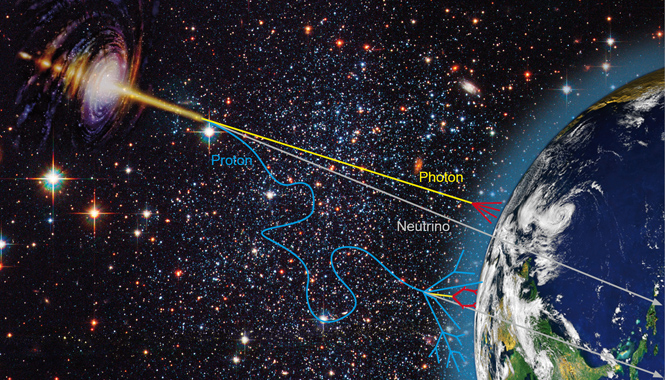
\includegraphics[width=0.6\textwidth]{./images/sources-detection.jpg}
  \caption{Möglicher Weg der dreier Klassen von Teilchen von der Quelle bis zu ihrer Detektion \cite{overview-detec}.}
\end{figure}

Auf die Erdatmosphäre treffen pro Sekunde und Quadratmeter durchschnittlich in etwa \num{e3} Teilchen~\cite{gaisser}.
Diese produzieren je nach Teilchenart und Energie Schauer, in denen viele Sekundärteilchen erzeugt werden. 
Je nach Teilchenart gibt es verschiedene Detektionsmöglichkeiten, wovon FACT eine erdbasierte Variante für $\gamma$-Quanten und Hadronen ist. 
Die verschiedenen kosmischen Teilchen lassen sich in drei verschiedene Klassen einteilen. 
Dabei zählt der Sonnenwind zu einer der ständigen Quellen, durch die geladene kosmische Strahlung auf die Erdatmosphäre trifft.

\section{Geladene kosmische Strahlung}
Geladene kosmische Strahlung besteht überwiegend aus Protonen, Heliumkernen und freien Elektronen. 
Aufgrund ihrer Ladung verliert sie jegliche Richtungsinformation durch intergalaktische Magnetfelder. 
Dies hat zur Folge, dass die Erde isotrop von geladener Strahlung getroffen wird.
Die geladene Strahlung tritt wesentlich häufiger auf, als die anderen beiden Klassen. 

\section{Photonen}
Photonen sind ungeladen, sodass eine Richtungsrekonstruktion mit ihnen möglich ist. 
Jedoch kommt es beim Eindringen der Teilchen in die Erdatmosphäre zur Schauerbildung, sodass die Richtungsrekonstruktion nicht ganz trivial ist. 
Dies kann umgangen werden, indem Satelliten in die Erdumlaufbahn gebracht werden, sodass der Cherenkov-Effekt erst gar nicht auftritt, wie es zum Beispiel beim Fermi Gamma-ray Space Telescope der Fall ist.

\section{Neutrinos}
Aufgrund ihrer elektrischen Neutralität sowie ihres geringen Wirkungsquerschnitts liefern Neutrinos Informationen über die Quellregionen. 
Dabei werden diese nicht durch galaktische Magnetfelder beschleunigt und somit geht ihre Richtungsinformation nicht verloren. 
Zum Nachweis von astrophysikalischen Neutrinos werden, aufgrund ihrer geringen Wechselwirkungswahrscheinlichkeit, große Detektorvolumina wie zum Beispiel das IceCube Experiment benötigt.
Da ein direkter Nachweis bis jetzt nicht möglich ist, wird beim IceCube Experiment der Cherenkov-Effekt im Eis genutzt, um über indirekte Strahlung Neutrinos nachzuweisen.

\chapter{FACT Grundlagen}
\begin{wrapfigure}[23]{R}[0pt]{0.45\textwidth}
  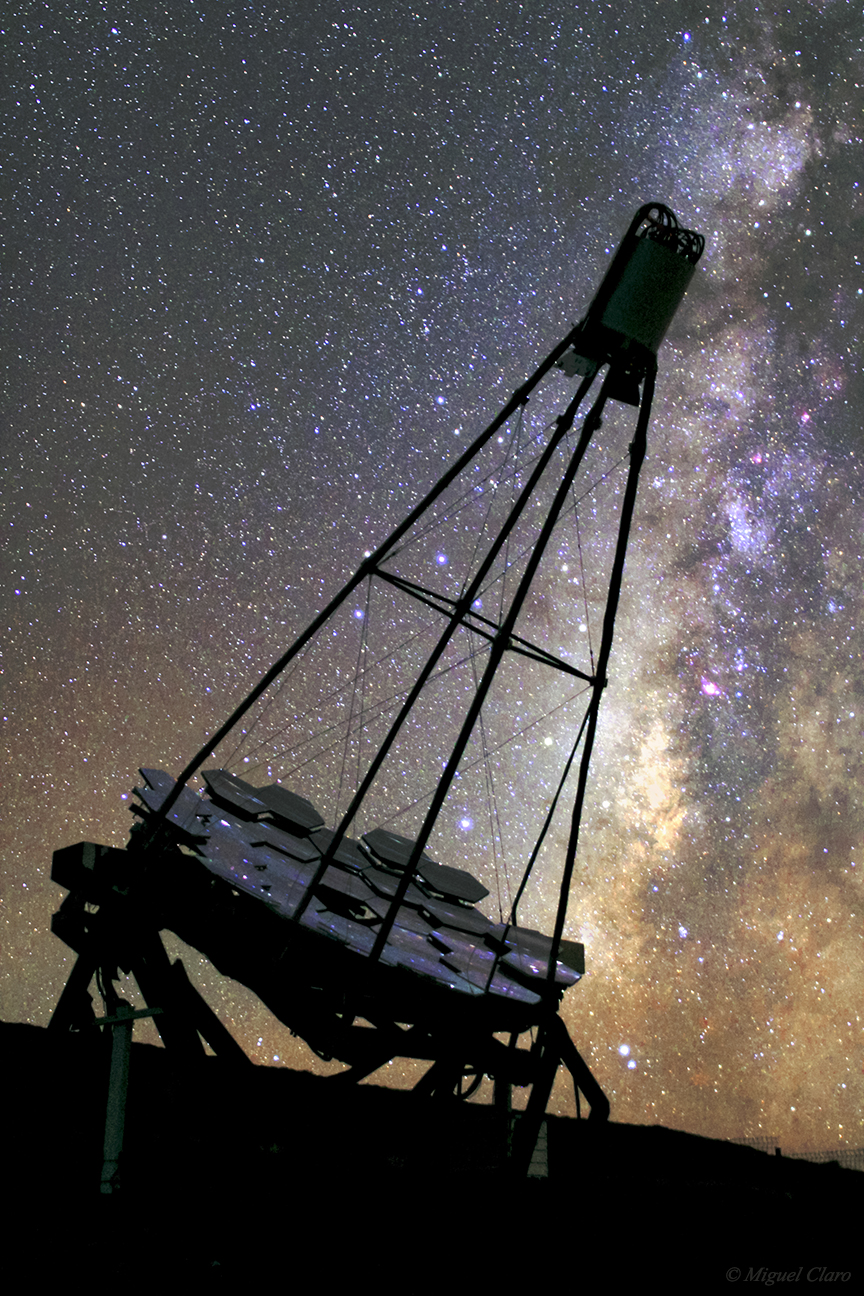
\includegraphics[width=0.45\textwidth]{./images/FACT.jpg}
  \caption{FACT in Observatiosposition \cite{factpic}}
  \label{fig:observ}
\end{wrapfigure}
Das FACT (First G-APD Cherenkov Telescope) dient der Überwachung von $\gamma$-Quellen, um bei erhöhter Aktivität, für genauere Observationen größere Telekope zu informieren. 
Desweiteren erprobt das Telekop die Nutzung von Silizium Photomultiplier (SiMPs) mit welchen es möglich ist, auch an Tagen mit starker diffuser Hintergrundstrahlung Quellen zu observieren. 

Auf einer Höhe von 2200 Meter über dem Meeresspiegel befindet sich das Cherenkov Teleskop auf der kanarischen Insel La Palma. 
Das Projekt entstand als ein Nachfolgerexperiment des übergebliebenen HEGRA CT3 Telskope, wobei die übergeblieben Spiegel aufbereitet und wiederverwertet werden.

Die 30 hexangonalen Spiegel bilden eine Gesamtspiegelfläche von \SI{9.51}{\meter\squared} bei einem Blickfeld von \SI{4.5}{\degree}. 
Die Spiegel sind seit der Neuausrichtung in der Davies-Cotton Design ausgerichtet \cite{design-detec}.
Dabei bilden die einzelnen Spiegel einen sphärisch ähnliche Fläche bei denen die Brennpunkte in die Kamera gelegt werden.

Als erstes Telskop seiner Zeit verwendet FACT, SiPMs anstelle von herkömlichen Photomultiplier Tubes. 
Halbleiterdetektoren lassen sich mit einer geringeren Operationsspannung (< \SI{100}{\volt}) betreiben und sind preiswerter als Photomultiplier, was die Gestaltung des Kameradesigns, als auch die Finanzierung vereinfacht. 
SiPMs sind aufgrund ihrer hohen Sensitivität dazu in der Lage einzelne Photonen zu detektieren, als auch bei Vollmond noch verwertbare Ergebnisse zu produzieren.
Dabei bilden 1440 Kamerapixel das Bild der Kamera, welche jeweils aus einem quadratischen Sensor und einem Plexiglasleiter bestehen. Die einzelnen Oberflächen der hexagonal zulaufenden Plexiglasleiter bilden dabei das Kamerabild.

\chapter{Entstehung von Cherenkov Schauern}
Trifft ein hochenergetisches Teilchen auf die Atmosphäre, löst dieses ein Schauer von Sekundärteilchen aus. Die Energie der erzeugten Sekundärteilchen ist stets geringer als das der einfallende Primärteilchen. Dabei wird zwischen zwei verschiedenen Arten von Schauern unterschieden. 

\textbf{Møglicher weise Tikz picture}

Trifft ein hochenergetisches $\gamma$-Quant auf die Atmosphaere, so wird es wahrscheinlich im Coloumbwall der Moleküle durch Paarerzeugung ein Elektronen-Positron-Paar erzeugen. 
Anschließend kann bei hinreichend großer Energie das Elektron durch Bremsstrahlung weitere Photonen erzeugen. 
\begin{eqnarray}
  \gamma \rightarrow& e^{+} + e^{-} \\
  e^{+} \rightarrow& e^{+'} + \gamma \\
  e^{-} \rightarrow& e^{-'} + \gamma 
\end{eqnarray}
Dieser Prozess ist solange fortlaufend bis, die Energie der Teilchen zu klein ist, ein neues Teilchenpaar zu erzeugen. 
Trifft ein geladenes kosmisches Teilchen in die Atmosphäre, so kann dieses über die starke Wechselwirkung, anders als beim elektromagnetischen Schauer, unterschiedliche Sekundärteilchen bilden. 
Dabei entstehen, unter anderem neue Hadronen, Mesonen und Myonen, welche wiederum zerstrahlen. 
\begin{eqnarray}
  \pi^{0} \rightarrow& \gamma + \gamma \\
  \pi^{+} \rightarrow& \mu^{+} + \nu_{\mu} \\
  \pi^{-} \rightarrow& \mu^{-} + \bar{\nu}_{\mu}
\end{eqnarray}
Entseht bei der Paarbildung schon früh ein $\pi^{0}$~Meson, so ist der Teilchenschauer kaum von dem eines $\gamma$-Quanten zu unterscheiden. 

Bewegt sich ein Teilchen schneller als die Lichtgeschwindigkeit in dem Medium polarisiert es dieses kurzzeitig. 
Dabei wird eine kohärente Schockwelle in Bewegungsrichtung abgestrahlt. Diese bilden ein Mach-Kegel aus, dessen Öffungswinkel $\theta$ von dem Brechungsindex $n$ des Mediums und der Phasengeschwindikeit der Welle abhängt.
\begin{equation}
  \cos  \theta = \frac{1}{\text{n} \beta}
\end{equation}
Wird in einem Cherenkov-Teleskop die Größe des Lichtkegels gemessen, bietet dies eine Möglichkeit, die Energie der Primärteilchen zu schätzen. 
\chapter{Observation}
\section{Bildgebene Paramter}
\begin{figure}[H]
  \centering
  \includegraphics[width=0.5\textwidth]{tikz/camera/camera.pdf}
  \caption{Hillas Parameter, anhand derer verschiedene Modelle zur Auswertung des Kamerabildes trainiert werden.}
\end{figure}
Fällt ein Schauer in das Teleskop, erzeugt dieses in der Kamera ein Bild. Nachdem Artefakte und äußere Einflüsse (noch mehr zu schreiben ?) bereinigt worden sind, wird anhand der Pixel, die auf den Cherenkovschauer zurückzuführen sind, die Hillas Parameter berechnet. 
Dazu wird im eine Gaußverteilung durch die Helligkeit der Pixel gefittet. 
Zu den Hillasparameter zählen:
\begin{itemize}
  \item \textbf{width/length:} Hauptachsen der Ellipse
  \item \textbf{size:} Anzahl an Pixel im Schauer
  \item \textbf{CoG:} Schwerpunkt des Schauers
  \item \textbf{Core of image:} Helligkeit der einzelnen Pixel
  \item \textbf{DISP:} Abstand zwischen Schwerpunkt des Schauers und der gemessenen Quellposition. Anhand der parameter width und length wird DISP abgeschätzt um die gemessene Quellposition zu ermitteln. Dabei gibt es zwei mögliche Vorzeichen, welche man durch die Observation der zeitlichen Konzentration der einzelenen Pixel im Schauer abzuschätzen versucht.
  \item \textbf{Source Position:} erwartete Quellposition
  \item \textbf{$\theta$:} Winkelzwischen der gemessenen und echten Quellposition
\end{itemize}
\section{Wobble Observation Strategy}
\begin{wrapfigure}[18]{L}[0pt]{0.53\textwidth}
  \includegraphics[width=0.5\textwidth]{images/wobble.pdf}
  \caption{Wobble observation muss noch zitiert werden. Theme dissertaion}
\end{wrapfigure}
Die Wobble Observation Strategy zeichnet aus, dass im Gegensatz zur klassischen Methode, nicht hintereinander On/Off Postionen beobachtet werden. 
Stattdessen wird die erwartete Quellpostion \SI{0.6}{\degree} neben die Kameraachse gelegt. 
Dies hat zur Folge, dass es mehrere Positionen mit dem selben Offest und Symmetrie zur Kameraachse gibt. 
Bei der Standardanalyse bei Fact können so neben der ON-Position, fünf Off-Positionen mit demselben Kippungswinkel zur Kameraachse gemessen werden. 
Somit ergibt sich für jedes Datensample jeweils ein $\theta_\text{on}$ und fünf $\theta_\text{off}$. 
Für sehr kleine $\theta$ Winkel kann oftmals geschlossen werden, dass das gemessene Teilchen aus Richtung der Quelle kam und vermutlich ein $\gamma$-Quant ist. 
Da der Hadron Untergrund isotrop in alle Richtungen verteilt auftritt, sollten bei hadronischen Schauern die Thetaverteilung in etwa gleichverteilt seien. 
Zu den Vorteilen dieser Methode zählen das keine extra OFF-Daten genommen werden müssen. 
Somit ist es möglich, die Messzeit der Quellaktivität zu maximieren. 
Desweiteren kann durch die gleichzeitige Datennahme davon ausgegangen werden, dass für die ON/OFF-Positionen annähernd die selben Wetterbedingungen gelten. 

\chapter{Überwachtes Maschinelles Lernen}
Zur Auswertung der Datenmengen von 300 GB bis 1 TB \cite{MaxNoethe} die FACT jede Nacht aufnimmt werden maschinelle Lernmethodenen verwendet. 
Maschinelles Lernen kann dazu genutzt werden, Muster und Strukturen auf Datensaetze zu erkennen und zukünftige Ereignisse hervorzusagen. 
Dabei wird zwischen überwachtem und unüberwachtem Training unterschieden.

Unüberwachtes Lernen kennzeichnet sich dadurch aus, dass versucht wird, auf dem Trainingsdatensatz spannende Muster zu erkennen.  

Ziel des überwachten Lernens ist es bei einem gegebenen Trainingsset welches aus Eingagsvariablen $X$ und Zielvariablen $y$ besteht Modelle zu finden, welche $X$ bestmoeglich auf $y$ abbilden. 
Zunächst muss dafur das Modell auf einen Datensatz trainiert werden. 
Dafür wird der Datensatz ($X$, $y$) in zwei Teile aufgeteilt, dem Trainings- und dem Testdatensatz. 
Dabei wird das Modell, auf den Trainingsdatensatz optimiert und anschließend auf dem Testdatensatz evaluiert. 
Dabei ist darauf zu achten, dass das Modell nicht nur den Trainingsdatensatz auswendig lernt (Übertraining), sondern allgemein genug bleibt auch ähnliche Datensätze genau vorherzusagen. 
Dies geschieht durch Beschränkung der Modelle. 
Durch Berechnung des Scores auf dem Testdatensatz welcher unabhänging von dem Trainingsmodell ist, kann geprüft werden, ob das Modell allgemein genug ist oder an Übertraining leidet.
\section{Entscheidungsbaum}
\begin{wrapfigure}[12]{R}[0pt]{0.5\textwidth}
  \centering
  \includegraphics[width=0.5\textwidth]{./tikz/tree/tree.pdf}
  \caption{Entscheidungsbaum der Tiefe 2 bei Gamma Handron Seperation}
\end{wrapfigure}
Ein Entscheidungsbaum besteht aus einem Wurzelknoten. Ausgehend von diesem wird durch Abfrage von verschiedenen Bedingungen eine Auswahl an Folgeknoten getroffen. 
In der Regel werden in der Datenanalyse, Binäre Entscheidungsbaume genutzt, sodass der Baum entsprechend an einem threshold wert die Daten an jedem Knoten in die zwei folgenden Knoten aufspaltet. 
Dieser Prozess wird solange durchgeführt bis ein Blatt erreicht wird. 
Die Anzahl an Knoten die durchlaufen werden bis das letzte Blatt errreicht wird, wird als Tiefe der Baeume bezeichnet.
Der Baum kann entsprechend verschiederner Kriterien gebaut werden.
Zu den gängigen gehört die Minimierung der Entropie oder des Gini-Indexes. 
Zu den Vorteilen eines Entscheidungsbaum zählt, dass dieser gut interpretierbar und nachvollziehbar ist. 
Desweiteren kommt es ohne Beschränkung schnell zum Übertraining.
\section{Random Forest}
Ein Random Forest besteht aus vielen schlechten Lernern.
Dabei werden mehrer Entscheidungsbäume unabhängig voneinander gebaut wobei der Erstellung eines Baumes immer nur eine Teilmenge aus allen Attributen gezogen wird.
Zur Klassifizierung wird anschließend eine Mehrheitsabstimmung durchgeführt.
Dadurch, dass die einzelnen Bäume Experten auf ihrem Teilgebiet sind und über die einzelnen Lerner gemittelt werden, ergibt sich ein Modell mit reduzierter Varianz im Gegensatz zum Entscheidungsbaum, welches robuster gegen Übertraining ist.
\section{extra boosted Decisiontree}

\section{Evaluieren}
Zum testen inwiefern sich die Modelle auf den Datensätze verhalten werden zweierlei Maße zu der Beurteilung von Klassifizierer benutzt.
\subsection{Receiver Operating Characteristic}
\begin{wrapfigure}[12]{R}[0pt]{0.4\textwidth}
  \centering
  \includegraphics[width=0.4\textwidth]{./Plots/roc_info.pdf}
  \caption{ROC Score zweier verschiedenen Modelle}
\end{wrapfigure}
Zum vergleich von verschiedenen Klassifizierung zweier Klassen ist der ``Receiver Operating Characteristic Curve'' ein Maß des Informationsgehalt. 
Dabei wird der die True Positive rate gegen die Fals Positive Rate aufgetragen fuer verschiedene confidencewerte. 
Für einen perfekten Klassifizier beträgt die Fläche unter der Kurve eins. 
Wird nur geraten strebt der Flächeninhalt gegen 1/2.
\subsection{Li und Ma Signifikanz}
Aufgrund der Begrenztheit der Dektorsensitivität muss bei der Analyse von möglichen Quellen sorgsam mit den Daten zur Bestimmung der Sicherheit einer Quelle umgegangen werden.
Dabei kann nicht das Signal einer Quelle isoliert gemessen werden. 
Stattdessen muss eine Sicherheit auf das Signals welches aus Richtung der Quelle $N_\text{on}$ und des Hintergrunds $N_\text{off}$ gegeben werden, dass das gemessene Signal nicht nur statistisches Rauschen ist.
Ein möglicher Anatz ist die Li and Ma Signifikanz, bei der über einen statistischen ``Null Hypothesen'' Test prüft ob das Signal $N_\text{S}$ nur ein Teil des Untergrunds $N_\text{B}$ ist. 
Aus dem Verhältniss der Messzeiten der On und Off position $\alpha$ wird die Hintergrundstrahlung berechnet. 
Aus Der Differenz der On Region und der Hintergrundrate lässt sich so die Signalrate bestimmen. 
Durch das Aufstellen der Maximum Liklihood Funktion und des anschließendem test ergibt sich fuer die Li and Ma Signifikanz.
\begin{equation}
S = \sqrt{2} \left( N_\text{on} \ln \left[ \frac{1+ \alpha}{\alpha}\left( \frac{N_\text{on}}{N_\text{on} + N_\text{off}} \right) \right] + N_\text{off} \ln \left[ \left( 1+ \alpha \right) \left( \frac{N_\text{off}}{N_\text{on} + N_\text{off}} \right) \right] \right)^{1/2}
\end{equation}

\chapter{Quellen}
In dieser Arbeit werden Datensätze von zwei verschiedenen Quellen verwendet. 
Beide dieser Quellen scheinen bereits gut verstanden und können zum vergleich zu anderen Arbeiten verwendet werden.
\section{Krebs Nebel}
In einer Entfernung von 6400 Lichtjahren befindet sich im Sternzeichen Stier der Überrest der ersten und letzten dokumentierten Supernovaexplosion, die auf das Jahr 1054 datiert ist. 
Die Überreste erstrecken sich über eine Fläche von 6 Bogenminuten Länge und 4 Bogenminuten Breite. 
In der Mitte des Krebs Nebels liegt ein Neutronenstern.
Aufgrund seines konstanten Strahlungsflusses ist der Krebsnebel eine Standard- und Kalibrierungsquelle in der Gammaastronomie.
Er gilt dabei als stärkste Quelle am Himmel. 
Viele wissentschaftliche Arbeiten nehmen diesen als Referenzwert um ihre Messwerte zu vergleichen. 

\section{Markarian 501}
Im Sternbild Herkules befindet sich in einer Entfernung von in etwa 500 Lichtfahren der Blasar Markarjan. 
In desse Zentrum befindet sich ein \num{0.9} bis \num{3.4} Milladrden Sonnenmassen schweres schwarzes Loch dessen Jet in Richtung Erde gerichtet ist.
Auch dieser gilt als einer der stärksten Gamma Strahlungsquellen.

\begin{figure}[H]
  \centering
  \includegraphics[width=\textwidth]{logos/theta_cut.pdf}
  \caption{}
  \label{fig:<+label+>}
\end{figure}

\begin{figure}[H]
  \centering
  \includegraphics[width=\textwidth]{logos/corr_sig_theta2.pdf}
  \caption{<+caption text+>}
  \label{fig:<+label+>}
\end{figure}

\begin{figure}
  \begin{subfigure}[b]{0.5\textwidth}
  \includegraphics[width=\textwidth]{logos/parameter_grid.pdf}
  \caption{<+caption text+>}
  \label{fig:<+label+>}
\end{subfigure}
\begin{subfigure}[b]{0.5\textwidth}
  \includegraphics[width=\textwidth]{logos/parameter_grid.pdf}
  \caption{<+caption text+>}
  \label{fig:<+label+>}
\end{subfigure}
\end{figure}

\begin{figure}[H]
  \centering
  \includegraphics[width=\textwidth]{logos/tikz/conf/conf.pdf}
  \caption{<+caption text+>}
  \label{fig:<+label+>}
\end{figure}<++>

\chapter{Zusammenfassung und Ausblick}
Das Ziel der Arbeit war, die Gamma/Hadron-Separation zu verbessern, indem anstelle der Monte Carlo simulierten Protonen gemessene Protonen zum Trainieren der Klassifizierer verwendet werden. 
Da diese eher dem gemessenen Untergrund ähneln, sollte eine bessere Klassifizierung erfolgen.

Weil FACT keine gemessenen Untergrund-Daten besitzt, muss ein Protonen-Datensatz aus dem Modifizieren einer bekannten Gamma-Quelle erstellt werden. 
Dies geschieht durch das Ausschneiden der Gamma-Quelle, mittels eines Schnitts, auf dem trennstärksten Parameter $\theta^{2}$.
Die Wahl des $\theta^{2}$-Schnitts liegen dabei folgende Überlegungen zugrunde:
Wird $\theta^{2}$ zu groß gewählt, kommt es dazu, dass Detektoreigenschaften signifikant werden und der Lerner einen großen Teil der $\theta^{2}$-Verteilung im Training nicht auswertet. 
$\theta^{2}$ darf auch nicht zu klein gewählt werden, da sonst noch verhältnismäßig viele Gamma-Ereignisse in dem erstellen Protonen-Datensatz sind.

Lerner welche auf simulierten Gamma- sowie Protonen-Events trainiert wurden, weisen niedrigere ROC-AUC-Werte auf, als welche die auf simulierte Gamma- und gemessenen Untergrund-Events trainierten wurden.
Eine mögliche Ursache dafür ist, dass die Modelle zwischen Simulation und gemessenen Ereignisse unterscheiden.

Diese Aussage lässt sich dadurch stützen, dass die Klassifizierer, die auf echten Daten trainiert wurden, zu niedrigeren Signifikanzen führen, als Lerner, die auf den Monte Carlo simulierten Daten trainiert wurden. 
Dies widerspricht der anfänglichen Vermutung, dass durch gemessene Daten die Separation verbessert werden kann. 
Zusätzlich weist ein weniger komplexer Baum wesentlich höhere Signifikanzen auf. 
In Verbindung mit seiner stark begrenzten Tiefe ist er damit möglicherweise nicht in der Lage, zwischen simulierten und gemessenen Protonen zu unterscheiden. 

Desweiteren konnte gezeigt werden, dass durch das Entfernen von Attributen, die einen hohen Monte Carlo Mismatch aufweisen, die Separation verbessert werden kann. 
Dies stützt die These, dass der Klassifizierer zwischen simulierten und echten Daten unterscheidet.

Letztendlich konnte die Gamma/Hadron-Separation nicht durch die Verwendung von gemessenen Protonen-Daten anstelle von simulierten im Trainingsdatensatz, verbessert werden. 

Ansatz weiterer Untersuchungen könnte die Nahme von Off-Daten seien.
Somit könnte auf den Schnitt um die Quellregion verzichtet werden. 
Desweiteren könnte durch die Verbesserung der Gamma Monte Carlo-Simulation, oder eines Modells welches robuster gegen Daten-Monte Carlo Mismatches bei gleicher TPR ist die Klassifikation verbessert werden.


\appendix
% Hier beginnt der Anhang, nummeriert in lateinischen Buchstaben
\chapter{Ein Anhangskapitel}

Hier könnte ein Anhang stehen, falls Sie z.B. Code, Konstruktionszeichnungen oder Ähnliches mit in die Arbeit bringen wollen. Im Normalfall stehen jedoch alle Ihre Resultate im Hauptteil der Bachelorarbeit und ein Anhang ist überflüssig.


\backmatter
\printbibliography

\cleardoublepage
\thispagestyle{empty}
\section*{Eidesstattliche Versicherung}
Ich versichere hiermit an Eides statt, dass ich die vorliegende Abschlussarbeit mit dem Titel \enquote{\thetitle} selbstständig und ohne unzulässige fremde Hilfe erbracht habe.
Ich habe keine anderen als die angegebenen Quellen und Hilfsmittel benutzt, sowie wörtliche und sinngemäße Zitate kenntlich gemacht. 
Die Arbeit hat in gleicher oder ähnlicher Form noch keiner Prüfungsbehörde vorgelegen.

\vspace*{1cm}\noindent
\begin{center}
  \begin{tabular}{@{}p{0.4\textwidth}@{\hspace{0.15\textwidth}}p{0.4\textwidth}@{}}
  \rule{\linewidth}{0.25pt}& \rule{\linewidth}{0.25pt}\\
  Ort, Datum & Unterschrift
  \end{tabular}
\end{center}

\subsection*{Belehrung}
Wer vorsätzlich gegen eine die Täuschung über Prüfungsleistungen betreffende Regelung einer Hochschulprüfungsordnung verstößt, handelt ordnungswidrig.
Die Ordnungswidrigkeit kann mit einer Geldbuße von bis zu \SI[round-mode=places, round-precision=2]{50000}{€} geahndet werden. 
Zuständige Verwaltungsbehörde für die Verfolgung und Ahndung von Ordnungswidrigkeiten ist der Kanzler/die Kanzlerin der Technischen Universität Dortmund. 
Im Falle eines mehrfachen oder sonstigen schwerwiegenden Täuschungsversuches kann der Prüfling zudem exmatrikuliert werden \mbox{(\S\,63 Abs. 5 Hochschulgesetz --HG--).}

Die Abgabe einer falschen Versicherung an Eides statt wird mit Freiheitsstrafe bis zu 3 Jahren oder mit Geldstrafe bestraft.

Die Technische Universität Dortmund wird ggf.\ elektronische Vergleichswerkzeuge (wie z.\,B.\ die Software \enquote{turnitin}) zur Überprüfung von Ordnungswidrigkeiten in Prüfungsverfahren nutzen. \\[\baselineskip]

\noindent Die oben stehende Belehrung habe ich zur Kenntnis genommen.\\[1cm]
\begin{center}
\begin{tabular}{@{}p{0.4\textwidth}@{\hspace{0.15\textwidth}}p{0.4\textwidth}@{}}
\rule{\linewidth}{0.25pt}& \rule{\linewidth}{0.25pt}\\
Ort, Datum & Unterschrift
\end{tabular}
\end{center}

\end{document}
